%=============================================================================
%  Section 4 -- Two orthogonal walls
%  Every number is a macro from macros.tex (authority: paper/NUMBERS.md).
%=============================================================================
\section{Two Orthogonal Walls}
\label{sec:two-walls}

Section~\ref{sec:cost-laws} measured one request at a time. A serving system
faces two independent pressures: how long each response must be, and how often
requests arrive. The cost laws answer the first. This section adds the second,
and finds that the two models fail along perpendicular axes --- the diffusion
model is indifferent to output length and collapses under arrival rate; the
autoregressive model is indifferent to arrival rate and collapses under output
length. Neither dominates; they are not on the same curve.

\subsection{Setup}
\label{sec:two-walls:setup}

We drive each server open-loop from an external Poisson arrival process at a
fixed offered rate $\lambda$ and report \emph{lag}: the wall-clock interval from
a request's arrival to its completion, which includes queueing and is therefore
the quantity a client actually experiences. This is deliberately not
closed-loop throughput: an open-loop driver does not slow down when the server
does, so the lag distribution reveals saturation rather than hiding it. Each
rate is run for 200\,s or 400 events, whichever comes first. Hardware, runtime
and data are as in Section~\ref{sec:cost-laws:setup}.

\subsection{The rate sweep}
\label{sec:two-walls:rate}

Table~\ref{tab:rate-sweep} sweeps $\lambda$ for both models.

\begin{table}[t]
  \centering
  \caption{Lag versus offered rate $\lambda$, open-loop Poisson arrivals.
    Dashes are rates not swept for that model; the two sweeps cover different
    ranges because the two saturation points differ by more than an order of
    magnitude. Note the serving asymmetry disclosed in
    Section~\ref{sec:two-walls:asymmetry}.}
  \label{tab:rate-sweep}
  \begin{tabular}{rrrrr}
    \toprule
    $\lambda$ (ev/s) & DG p50 lag (ms) & DG p99 (ms) & AR-3B p50 lag (ms) & AR-3B p99 (ms) \\
    \midrule
    1    & \dgLagOne & \needsnum{dgPNineNineOne} & \arLagOne & \needsnum{arPNineNineOne} \\
    1.5  & \needsnum{dgLagOneFive}  & \needsnum{dgPNineNineOneFive}  & --- & --- \\
    2    & \needsnum{dgLagTwo}      & \needsnum{dgPNineNineTwo}      & --- & --- \\
    2.5  & \needsnum{dgLagTwoFive}  & \needsnum{dgPNineNineTwoFive}  & --- & --- \\
    4    & \needsnum{dgLagFour}     & \needsnum{dgPNineNineFour}     & \needsnum{arLagFour} & \needsnum{arPNineNineFour} \\
    8    & --- & --- & \needsnum{arLagEight}     & \needsnum{arPNineNineEight} \\
    32   & --- & --- & \needsnum{arLagThirtyTwo} & \needsnum{arPNineNineThirtyTwo} \\
    64   & --- & --- & \needsnum{arLagSixtyFour} & \needsnum{arPNineNineSixtyFour} \\
    96   & --- & --- & \needsnum{arLagNinetySix} & \needsnum{arPNineNineNinetySix} \\
    128  & --- & --- & \needsnum{arLagOneTwoEight} & \needsnum{arPNineNineOneTwoEight} \\
    \bottomrule
  \end{tabular}
\end{table}

The diffusion model saturates at $\lambda \approx \dgKneeLo$--$\dgKneeHi$~ev/s.
Below the knee its lag tracks its \dgBase{}\,ms service time closely; above it,
lag grows without bound within the measurement window and requests are
abandoned. The autoregressive model saturates at
$\lambda \approx \arKneeLo$--$\arKneeHi$~ev/s, roughly $\kneeRatio\times$ more
offered load. Their p50 curves cross at $\lambda \approx \rateCrossover$~ev/s:
below that rate the diffusion model has the lower lag (\dgLagOne{}\,ms against
\arLagOne{}\,ms at $\lambda=1$), and above it the autoregressive model does, by
a margin that widens catastrophically rather than gradually. As noted among our
threats to validity, the \emph{location} of each knee is the result here; the
exact tail milliseconds past saturation are transient-windowed (300-event
windows with a 45\,s drain) and should not be read as steady state.

\subsection{The saturation point is predicted by queueing theory alone}
\label{sec:two-walls:mdone}

The diffusion knee is not an empirical curiosity, and it is worth stating as a
result rather than an aside. Section~\ref{sec:cost-laws} established that the
diffusion model's service time is essentially deterministic inside one canvas:
\dgBase{}\,ms, independent of the content and of the output length. A server
with Poisson arrivals and deterministic service is an M/D/1 queue, which is
stable exactly for $\lambda < \mu$ where $\mu$ is the reciprocal of the service
time. Substituting the service time from Eq.~\eqref{eq:law-dg} and nothing else
gives
%
\begin{equation}
  \mu \;=\; \frac{1}{T_{\mathrm{DG}}(L \le \dgCanvas)} \;\approx\; \mdOneMu~\text{ev/s}.
  \label{eq:mdone}
\end{equation}
%
The measured knee is $\dgKneeLo$--$\dgKneeHi$~ev/s. The prediction lands inside
the measured interval, and it uses no fitted parameter from
Section~\ref{sec:two-walls:rate} --- only the single-request service time from
Section~\ref{sec:cost-laws}. In other words, the capacity of a serialized
diffusion server is fully determined by its service time, because there is no
batching term to add to it. This is the first place where the mechanism of
Section~\ref{sec:mechanism} shows through: for the autoregressive model no such
single-parameter prediction is possible, since its capacity is set by how many
requests the scheduler can co-resident, not by how long one request takes.

\subsection{The joint grid: two orthogonal walls}
\label{sec:two-walls:grid}

Sweeping $\lambda$ and $L$ separately understates the structure. We therefore
ran a uniform grid, $L \in \{64,128,256,512\}$ crossed with
$\lambda \in \{1,2,4,8,16\}$~ev/s, on both models. Figure~\ref{fig:joint-grid}
is the result and is the central picture of this paper.

The two lag surfaces are close to perpendicular. Diffusion lag is flat in $L$
--- as Eq.~\eqref{eq:law-dg} requires, since the whole grid up to $L=256$ lives
inside one canvas --- and walls in $\lambda$ at the knee of
Section~\ref{sec:two-walls:mdone}. Autoregressive lag is flat in $\lambda$
across the entire swept range --- continuous batching absorbs the offered load
--- and walls in $L$, at \arSlope{}\,ms for every token added. Each model is
immune to precisely the axis that destroys the other.

The consequence is a bounded win region rather than a ranking: the diffusion
model is preferable when $\lambda \lesssim \winRegionRate$~ev/s
\emph{and} $L \ge \winRegionLen$ tokens, reaching
\needsnum{winRegionSpeedup}$\times$ lower lag at the corner ($\lambda=1$,
$L=512$) and tying at $L=64$. Outside that region the autoregressive model wins,
and outside it in the $\lambda$ direction it wins by margins that make the
comparison uninteresting. The practical reading is that a served diffusion model
is a fit for workloads that are slow and verbose --- long structured
documents arriving at human rather than machine rates --- and a poor fit for
anything resembling high-volume telemetry.

\begin{figure}[t]
  \centering
  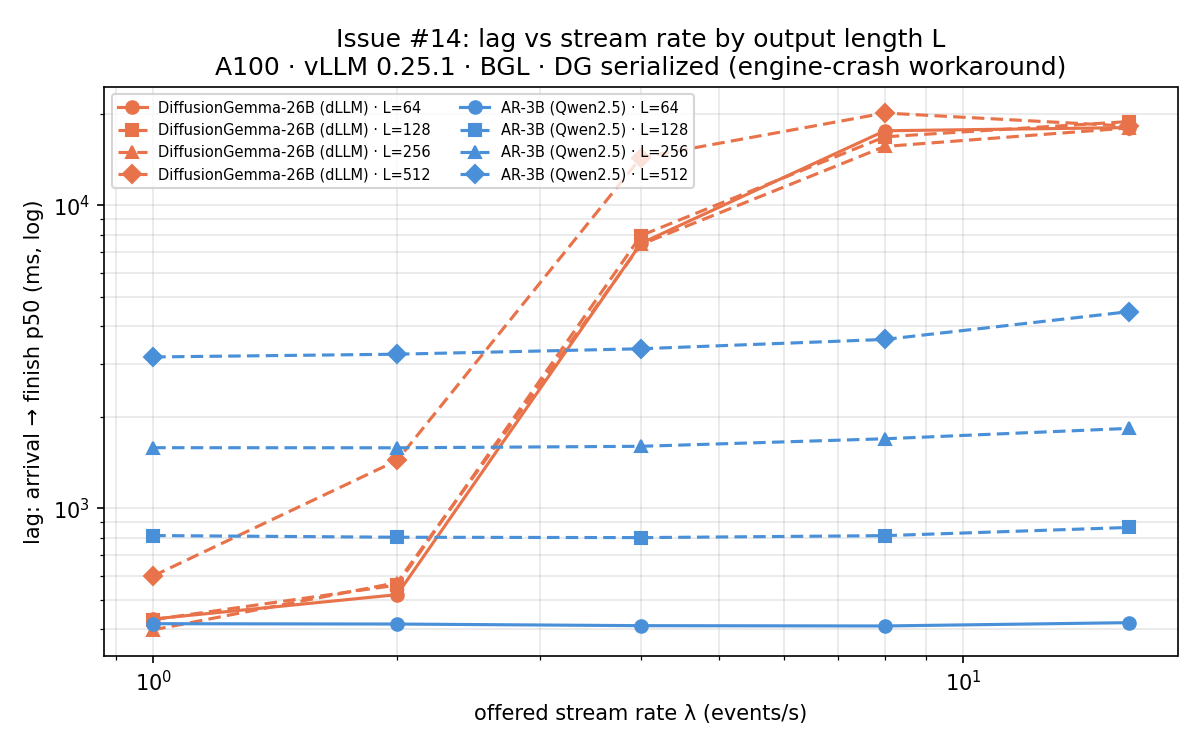
\includegraphics[width=0.95\textwidth]{../results/joint_rate_lag.png}
  \caption{\textbf{Two orthogonal walls.} Lag over the joint grid
    $L \in \{64,128,256,512\}$ tokens $\times$ $\lambda \in \{1,2,4,8,16\}$~ev/s
    for both models. Diffusion lag is flat in $L$ and walls in $\lambda$;
    autoregressive lag is flat in $\lambda$ and walls in $L$. The diffusion
    win region is $\lambda \lesssim \winRegionRate$~ev/s and
    $L \ge \winRegionLen$ tokens.
    \textbf{Serving asymmetry, disclosed:} \modelDG{} is served with
    \texttt{-{}-max-num-seqs 1} (serial) while \modelARthree{} runs vLLM's
    default 256-way continuous-batching scheduler. The asymmetry is forced by an
    engine defect, not chosen --- see Section~\ref{sec:two-walls:asymmetry}.
    \todo{chart will be regenerated for print -- static render, shared colour
      scale across both panels, log axis on lag, and the win region outlined.}}
  \label{fig:joint-grid}
\end{figure}

\subsection{Serving asymmetry: mandatory disclosure}
\label{sec:two-walls:asymmetry}

The two models in Table~\ref{tab:rate-sweep} and Figure~\ref{fig:joint-grid} are
not served under identical scheduler settings, and the difference favours the
autoregressive model. \modelDG{} is served with \texttt{-{}-max-num-seqs 1},
which serializes it: at most one request is in flight at any time.
\modelARthree{} is served with vLLM's default 256-way continuous-batching
scheduler. Reported this way, the diffusion knee in
Section~\ref{sec:two-walls:rate} is partly a statement about a scheduler
setting and not only about an architecture.

We did not choose this asymmetry. In vLLM 0.25.1 the DiffusionGemma runner
crashes at \texttt{diffusion\_gemma.py:96} with a tensor-size mismatch
(``size 257 vs 256'') as soon as \texttt{num\_running\_reqs=2} places two
canvases in different denoising phases inside one batch; the engine dies rather
than degrading. Serial serving is the model's only stable configuration in this
runtime. The failure is tracked upstream as
\texttt{vllm-project/vllm\#50699}, where the maintainers' analysis attributes it
to self-conditioning/residual misalignment across mixed-phase canvases; the
proposed fix, \texttt{\#51994}, in the maintainers' own words \emph{``trades the
crash for serialization''}, and no parallel denoising batching is planned ahead
of the MRV2 runner rewrite (\texttt{\#52015}). Our reproduction is posted on
that issue.

Two things follow, and we state both. First, serialized serving is currently the
diffusion model's production-relevant mode in this runtime --- a deployment
today gets the numbers in Table~\ref{tab:rate-sweep}, not some hypothetical
batched numbers, so these are the honest figures for a system built on this
stack. Second, they are nevertheless not an architectural upper bound on
diffusion serving, and nothing in this section establishes one. The argument
that the batching ceiling is architectural rather than a defect of this
particular runner is made in Section~\ref{sec:mechanism}, and it rests on a
second, independent runtime --- not on these measurements.
